\section{Algorithm Output and Testing}
% Writing code: Make it run. Make it correct. Make it fast.
My implementation of the linear-Gaussian binary latent feature model with the IBP prior generates the results in images and traceplots. The simulated dataset contains four latent features (see Figure~\ref{fig:images}), and my code reveals all of them in Figure~\ref{fig:imageresults}. Note that my Gibbs sampler is sensitive to the random seed settings, and using another random seed in the code initialization reveals five (instead of four) latent features in Figure~\ref{fig:imageresultsK5}, three of which are the linear combinations of two latent features.\\ 

The traceplots in Figure~\ref{fig:plotresults} show my Gibbs sampler is converging: $K_+$ fluctuates between 5 and 8; the IBP parameter $\alpha$ is within (0.2,3.0); $\sigma_X$ converges to the true value 0.5; $\sigma_A$ oscillates around 0.4. A total of 1000 Gibbs sampling iterations were performed, but the values started to converge at the 100th iteration.

\begin{figure}[!ht]
\centering
    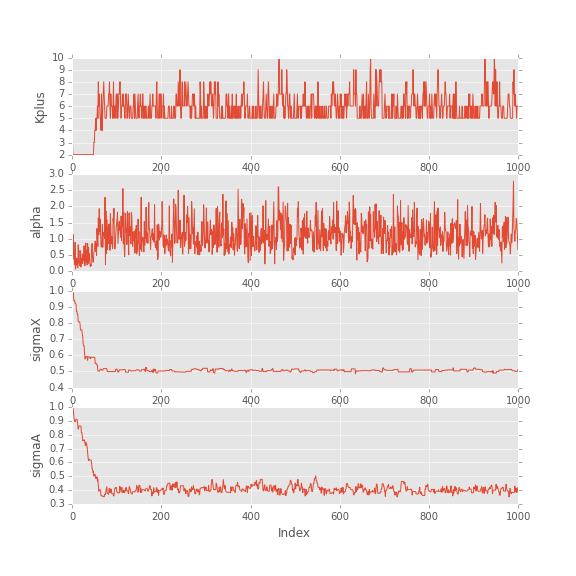
\includegraphics[width=0.65\linewidth]{IBP_plot_results.png}
    \vspace{-20pt}
    \caption{The traceplots for $K_+, \alpha, \sigma_X, \sigma_A$}
    \label{fig:plotresults}
\end{figure}

\begin{figure}[!ht]
\centering
    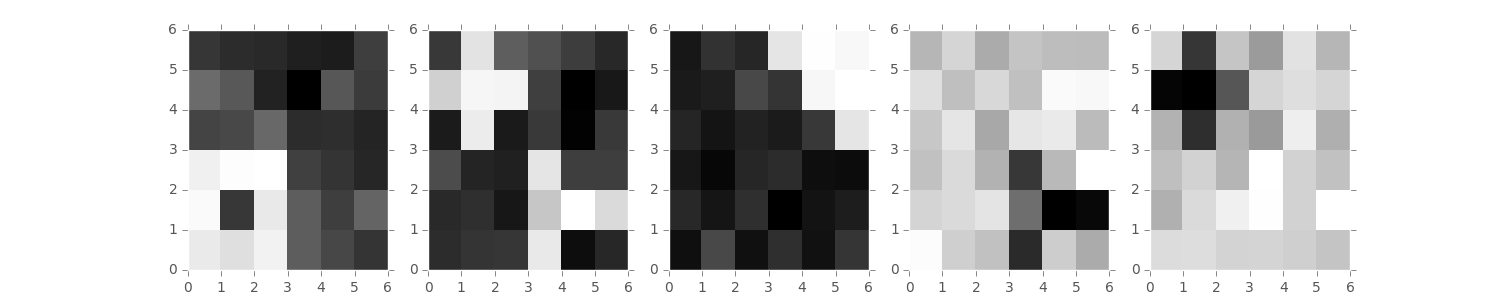
\includegraphics[width=\linewidth]{IBP_image_results.png}
    \caption{Simulated dataset: My results}
    \label{fig:imageresults}
\end{figure}

\begin{figure}[!ht]
\centering
    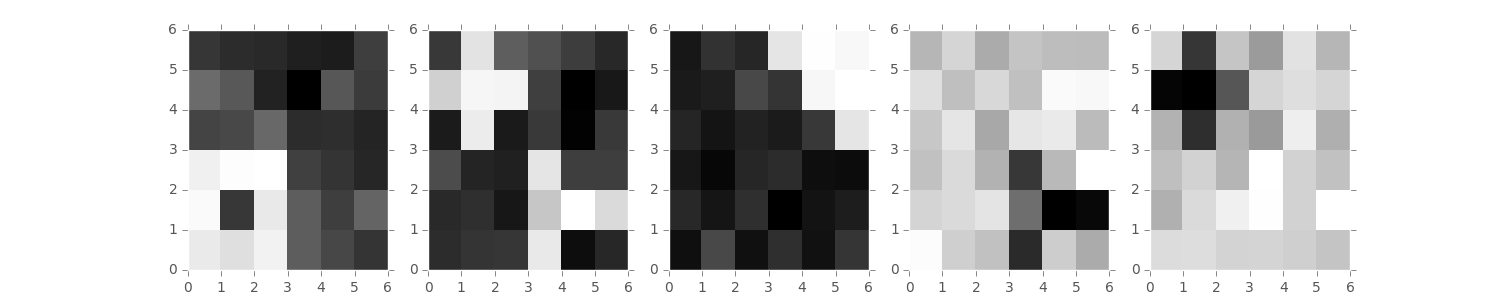
\includegraphics[width=\linewidth]{IBP_image_results_K5.png}
    \caption{Simulated dataset: My results with another random seed}
    \label{fig:imageresultsK5}
\end{figure}

\subsection{Code Testing}

Code testing is performed by various methods. In the IBP prior, the \texttt{assert} command is used to verify $\frac{m_k}{i}$ to be a probability, i.e. between 0 and 1 -- because the $i$th ($i > 2)$ customer takes dish $k$ with probability $\frac{m_k}{i}$ in the IBP algorithm. In many parts of my code, I used \texttt{np.dot} from \texttt{numpy} to do matrix multiplications even when the size of matrices is small, instead of multiplying each column/row one by one. In this way, the dimensions in matrix multiplications are assured to match each other.\\

For unit testing, the functions \texttt{calcM}, \texttt{calInverse\_orig}, \texttt{calInverse} are tested by an external file. The first function \texttt{calcM} calculates $\mathbf{M} = (\mathbf{Z}^T\mathbf{Z}+\frac{\sigma_X^2}{\sigma_A^2}\mathbf{I})^{-1}$, and the correctness is ensured by showing that $\mathbf{M}\mathbf{M}^{-1} = \mathbf{I}$. Note that \texttt{calcM} involves inversion, so it may be a bottleneck of my IBP code.\\

Therefore, I attempted to expedite the calculation of $\mathbf{M}$ by using Equations (51)-(54) in Griffiths' and Ghahramani's paper~\cite{griffiths2005detailed}, when only one value of the whole matrix $\textbf{Z}$ is changed. Theoretically, this method below allows us to efficiently compute $\mathbf{M}$ when the $i$th row of $\mathbf{Z}$ (denoted as $\mathbf{z_i}$) has changed:
\begin{gather}
\text{Define } \mathbf{M}_{-i} = (\sum_{j \neq i}\mathbf{z}^T_j \mathbf{z}_j + \frac{\sigma_X^2}{\sigma_A^2}\mathbf{I})^{-1} \\
\mathbf{M}_{-i} = (\mathbf{M}^{-1} - \mathbf{z}^T_i \mathbf{z}_i)^{-1} 
= \mathbf{M} - \dfrac{\mathbf{M}\mathbf{z}^T_i \mathbf{z}_i\mathbf{M}}{\mathbf{z}_i\mathbf{M}\mathbf{z}^T_i - 1} \\
\mathbf{M} = (\mathbf{M}_{-i}^{-1} - \mathbf{z}^T_i \mathbf{z}_i)^{-1} 
= \mathbf{M}_{-i} - \dfrac{\mathbf{M}_{-i}\mathbf{z}^T_i \mathbf{z}_i\mathbf{M}_{-i}}{\mathbf{z}_i\mathbf{M}_{-i}\mathbf{z}^T_i + 1}
\end{gather}

The function \texttt{calInverse\_orig} returns $\mathbf{M} = \mathbf{M}_{-i} - \dfrac{\mathbf{M}_{-i}\mathbf{z}^T_i \mathbf{z}_i\mathbf{M}_{-i}}{\mathbf{z}_i\mathbf{M}_{-i}\mathbf{z}^T_i + 1}$, and the function \texttt{calInverse} returns $\mathbf{M} = (\mathbf{M}_{-i}^{-1} - \mathbf{z}^T_i \mathbf{z}_i)^{-1} $ just for comparison results. One drawback of this method is that numerical errors can be accumulated, leading to wrong results. Therefore, a full rank update of $\mathbf{M}$ should be performed occasionally. In fact, unit testing shows that they give different results from the original \texttt{calcM} function, and using the \texttt{calInverse} functions makes $K_+$ stuck at 2, which is incorrect.\\

I also tested the log-likelihood for the Poisson distribution in my IBP code by showing the probability mass function $f(x)$ below integrates to 1.
\begin{gather}
x \sim \text{Pois}(\lambda): f(x) = \dfrac{\lambda^x}{x!} e^{-\lambda}, x = 0,1,2,3,\cdots \\
\log f(x) = x \log \lambda - \lambda - \log(x!)
\end{gather}
Therefore, $\exp \log f(x) = 1$ is approximated by $\sum^{20}_{x=0}f(x)$ in the unit testing code.\\